\documentclass[12pt,letterpaper]{report}
%for roman numeral sectioning
\renewcommand{\thesection}{\Roman{section}} 
%\renewcommand{\thesubsection}{\thesection.\Roman{subsection}}


%Set depth of numbering
\setcounter{secnumdepth}{1} % only chapter and sections will be numbered
\setcounter{tocdepth}{2}    % entries down to \subsubsections in the TOC
%make 1 inch margins.

\usepackage[margin=1in]{geometry}

%to fix unordered numbering when using captions.
%\usepackage{notoccite}

%page number top right (comment it all out if you want page num on bottom middle)
%\usepackage{fancyhdr}
%\pagestyle{fancy}
%\renewcommand{\headrulewidth}{0pt}
%\fancyhf{}
%\fancyhead[R]{\thepage}


%underline section titles
%\usepackage[explicit]{titlesec}
%\usepackage{ulem}
%
%\titleformat{\section}
%  {\normalfont\large\itshape}{\thesection}{1em}{\uline{#1}}
  
\usepackage[latin1]{inputenc}
\usepackage{amsmath}
\usepackage{amsfonts}
\usepackage{amssymb}
\usepackage{setspace}
%\usepackage{tocloft}
\usepackage[compact]{titlesec}
\usepackage[parfill]{parskip}

\usepackage{graphicx}
\usepackage{wrapfig}

\usepackage[super,comma]{natbib}

%
\usepackage{titling}

\usepackage{pdfpages}

%To remove square brackets
\usepackage{ifthen}
\makeatletter
\renewcommand\@cite[2]{%
Ref.~#1\ifthenelse{\boolean{@tempswa}}
{, \nolinebreak[3] #2}{}
}
\renewcommand\@biblabel[1]{#1.}
\makeatother

%for quotes
\usepackage [english]{babel}
\usepackage [autostyle, english = american]{csquotes}
\MakeOuterQuote{"}

%This format looks alright.
\bibliographystyle{lastfirstabbrunsrtednat}

% Remove brackets from numbering in List of References
%\makeatletter
%\renewcommand{\@biblabel}[1]{\quad#1.}
%\makeatother

%Set the format of the titles
\titleformat{\chapter}[display]
{\singlespacing\bfseries\Huge}
{\titlerule\filright\Large\chaptertitlename\ \Large\thechapter}
{0pt}
{\filright}
[\titlerule]
\titlespacing*{\chapter}{0pt}{0pt}{*2}

\renewcommand{\thepage}{\roman{page}}% Roman numerals for page counter
\doublespacing


%Change behavior of the contents
\makeatletter
\renewcommand*\@makechapterhead[1]{%
  %\vspace*{50\p@}%
  {\parindent \z@ \raggedright \normalfont
    \ifnum \c@secnumdepth >\m@ne
        \huge\bfseries \@chapapp\space \thechapter
        \par\nobreak
        \vskip 20\p@
    \fi
    \interlinepenalty\@M
    \centering \Huge \bfseries #1\par\nobreak
    \vskip 40\p@
  }}
\renewcommand*\@makeschapterhead[1]{%
  %\vspace*{50\p@}%
  {\parindent \z@ \raggedright
    \normalfont
    \interlinepenalty\@M
    \centering \Huge \bfseries  #1\par\nobreak
    \vskip 40\p@
  }}
  %This adds dots to the chapters
  \renewcommand*\l@chapter{\@dottedtocline{1}{0em}{1.5em}}
  \renewcommand*\l@subsection{\@dottedtocline{2}{5em}{3.2em}}
\makeatother

\begin{document}
%We need a cover page too ;(

\title{Comparative Report of the Oxford Nanopore DNA Sequencing Technology and Current Sequencers}
\author{Molly LoSchiavo, Corianne Galloway, Kevin Boehme}
\date{}
\maketitle

%Title Page
%Title page
\title{Comparative Report of the Oxford Nanopore DNA Sequencing Technology and Current Sequencers}
\author{Submitted to \\
Sister Hadden \\
for \\
English 316 \\
Brigham Young University \\
Provo, Utah \\
\today \\
\\
\\
by \\
Molly LoSchiavo, Corianne Galloway, Kevin Boehme}
\date{}
\maketitle

\pagenumbering{gobble}
%Letter of Transmittal
%Just need to write it the old fashion way.
\begin{center}
\Huge\textbf{Letter of Transmittal}
\end{center}
\begin{flushleft}
\today \\[1\baselineskip]
\begin{singlespace}
English 316 \\
Sister Hadden \\
3004 JKB \\
Brigham Young University \\
Provo, UT 84602 \\
(801) 422-4704 \\[1\baselineskip]
\end{singlespace}
Dear Sister Hadden, \\[1\baselineskip]
As a group, we are prepared to submit a copy of the Technical Report assignment for English 316 to you and our peers.\\ [1\baselineskip]
The purpose of the report is to provide a comparison of current DNA sequencing technologies with the new Oxford Nanopore technology. We focused on three of the "next-generation" sequencing technologies to use for comparison: Illumina, Pacific Biosciences, and Ion Torrent. To compare these technologies, we concentrated on three criteria to determine the best recommendation for the most efficient technology based on cost per megabase, time per run, and output per run. \\[1\baselineskip]
Please take time to look over our report. We are anxious for feedback, so we can make the necessary improvements. If you have questions or comments please contact us at coric8@gmail.com, mollyloschiavo@gmail.com, or kevinlboehme@gmail.com. \\ [1\baselineskip]
Sincerely,\\[1\baselineskip]
Corianne Galloway, Molly LoSchiavo, Kevin Boehme
\end{flushleft}

\clearpage


%Table of Contents
%change level of indendation
%\setlength{\cftbeforetoctitleskip}{-2em}
%\cftsetindents{subsection}{.75in}{.75in}
\renewcommand*\contentsname{Table of Contents}
\setcounter{page}{3}
\renewcommand{\thepage}{\roman{page}}% Roman numerals for page counter
%\renewcommand{\cftpartleader}{\cftdotfill{\cftdotsep}} % for parts
%\renewcommand{\cftchapleader}{\cftdotfill{\cftdotsep}} % for chapters
\tableofcontents
\clearpage

%List of figures
%\thispagestyle{empty}

\addcontentsline{toc}{chapter}{\listfigurename}
\listoffigures
\begingroup
\let\clearpage\relax
\addcontentsline{toc}{chapter}{\listtablename}
\listoftables
\endgroup
\clearpage

%List of Tables
%\addcontentsline{toc}{chapter}{\listtablename}
%\listoftables
%\clearpage

%Abstract
\addcontentsline{toc}{chapter}{Abstract}
\begin{center}
\Huge\textbf{Abstract}
\end{center}
This report is a comparative analysis of desktop DNA sequencers: Oxford Nanopore (MinION), Illumina (MiSeq), Ion Torrent (PGM), and Pacific Bioscience (RS II). Oxford Nanopore is a new technology that is garnering a lot of hype in the media. Our goal is to compare the results of Oxford Nanopore's desktop DNA sequencer (MinION) with the three most popular DNA sequencers in the market. We aim to determine 1) if the MinION measures up to the hype it's received and 2) which sequencing technology is the most efficient in terms of money, time, and output. 

We collected data from studies that compared the older sequencing technologies as well as recent data from experiments which used the Oxford Nanopore sequencer. With this data, we made comparisons between the DNA sequencers based on cost per megabase, time per run, and output per run. Our results indicate that Oxford Nanopore costs about 3 times more than the next most expensive sequencer (PacBio) and 10 times more than the cheapest sequencer (Illumina). Oxford Nanopore also has the longest time per run and the second-lowest output per run of all the technologies. In our analysis, we combined the time per run and output per run measurements to formulate a new standard, throughput, or output per hour. We found that the MinION also has the lowest throughput of all the technologies. 

Our conclusion is that the Oxford Nanopore technology performs far worse in terms of time, money, output, and throughput than the established sequencing technologies. We further determine that Illumina's MiSeq is the most efficient desktop sequencer, capable of sequencing DNA cheaper and faster than any other desktop machine included in the study.

\clearpage

%Start the report
\setcounter{page}{1}
\renewcommand{\thepage}{\arabic{page}}% Roman numerals for page counter

%Title
\begin{center}
\textbf{\Large{Comparative Report of the Oxford Nanopore DNA Sequencing Technology and Current Sequencers}}
\end{center}

\section{Introduction}
The subject of our project is comprised of the up-and-coming Oxford Nanopore DNA sequencing technology and the most popular \textit{next-generation DNA sequencers} (see Glossary). As for the purpose of our study, we aim to provide a digestible and practical comparison of current sequencing technologies with that of the new Oxford Nanopore technology to determine if Oxford Nanopore deserves all of the hype it's been receiving and to determine which technology's desktop unit is the most efficient in terms of money, time, and output.

The scope of this study involves the comparison of Oxford Nanopore's desktop unit, the MinION, to the three most popular desktop next-generation DNA sequencing machines: Illumina's MiSeq, Ion Torrent's PGM, and Pacific Biosciences' (PacBio) RS II. To identify which of these technologies is most efficient, we focused on three main criteria: cost per \textit{megabase}, time per run, and output per run. 

The development of our project consisted of three steps: research, analysis, and solution. We first collected data and information regarding the three criteria mentioned above as well as any other research previously done on this subject. This information helped us formulate our background material as well as lay a foundation for analysis. We gathered this information from prominent next-generation sequencing technology websites such as www.allseq.com, www.biomedcentral.com, and www.illumina.com. In addition, we found studies from reputable biotechnology journals such as Nature Biotechnology, Science, and Genome Research. We also found information regarding recent results from Oxford Nanopore's MinION unit in a study performed by Quick, et al., as well as recent installments on its development and implementation \cite{Quick}. With this data, we created visual comparisons between the technologies based on the criteria mentioned in the scope of our project. In addition, we combined the time per run and output per run measurements to formulate a new standard, throughput, or output per hour. We felt that this new measurement was more indicative of the productivity of each machine. After we completed our analysis, we formulated a recommendation for the overall most efficient sequencing technology.

We believe that our work will prove useful to a variety of groups. For example, the field of bioinformatics deals with DNA sequence processing, and any potential "game-changing" technology (i.e. Oxford Nanopore) will be of intense interest to everyone in this field. Health professionals and pharmaceutical companies will be interested in this study if the results indicate a potential for rapid clinical applications by significantly reducing costs or time for sequencing. In addition, many individuals in the biotechnology arena follow sequencing technologies closely, and this study may provide tractable information to them.

\section{Background}

\subsection{Introduction to Sequencing}

\textit{DNA} is a molecule that is commonly referred to as "the blueprint of life". That is because the DNA found in just one of your trillions of cells contains all of the information needed to make, grow, and operate your body! This information is stored in the form of DNA sequence. DNA is composed of four kinds of molecules called \textit{nucleotides}: adenine, guanine, cytosine, and thymine. For simplicity, these nucleotides are referred to as A, G, C, and T, respectively. DNA sequence is the order in which these nucleotides occur. Within the 3 billion nucleotides that make up the human \textit{genome} lie many of the answers to our questions about ancestry, life processes, and diseases such as cancer, Alzheimer's, and autism.

The first efforts to unearth this valuable sequence began in the 1970s. At this time, the prevailing sequencing technology (Sanger sequencing) was primitive and too expensive to sequence anything larger than a couple hundred thousand nucleotides long. However, as new technologies emerged, and public interest increased over the following decades, the world of DNA sequencing experienced an event that changed it forever: The Human Genome Project. 

The mapping of the human genome was one of the largest collaborative projects in human history. With the presentation of this invaluable data to the public came a rush of new DNA sequencing technology. Many universities, research facilities, and private companies wanted to hitch a ride on the coattails of this new, exciting opportunity to perhaps get their own chance at changing the world. Through this, many brand-name technologies emerged such as Illumina, Ion Torrent, and PacBio. These technologies came to be known as "next-generation sequencing technologies" because of their technological advancement as compared to earlier sequencing technologies like Sanger sequencing \cite{Shendure}. Although much progress has been made in the field of genomics, researchers are still eager for cheaper, faster, and better sequencing technologies. Specific goals that the field has set include reducing the cost of sequencing an individual's genome to less than \$1,000 and advancing medical and genomic research to someday realign the medical diagnostic framework which will allow patients to receive treatments specific to their genomic makeup \cite{Salto-Tellez}. While current technologies have gotten us close to achieving these goals, there still remains room for improvements.

Oxford Nanopore is an up-and-coming sequencing technology that claims to be leading the world to a \$1,000 genome sequence with longer read lengths and shorter run time due to the fundamental design of the technology \cite{Maitra}. The advancement in technology that the new sequencing method uses (called strand sequencing) is what put Oxford Nanopore in the "third-generation sequencing technologies" category. We will now introduce each technology individually.

	
\subsection{Illumina}

Nucleotides perform base-pairing between strands of DNA. In \textit{base-pairing}, A and T only pair with each other, and C and G only pair with each other. Using this, Illumina employs "sequencing by synthesis" to sequence DNA. Sequencing by synthesis works by first isolating a single strand of DNA. Next, all four nucleotides are introduced to the strand. Because of base-pairing, only the nucleotide that matches the sequence will attach to the strand. On this newly attached nucleotide is a \textit{fluorophore}. Fluorophores fluoresce a specific color when activated by a laser. Each nucleotide is given a separate color. In Figure 1, T is red, G is green, C is yellow, and A is blue. After the nucleotide base-pairs to the DNA strand, the Illumina machine flashes a laser, and a camera records what color fluoresces. This tells the machine which nucleotide was attached to the strand. This process is then repeated until the entire DNA strand has been sequenced and recorded.

\begin{wrapfigure}{r}{0.6\textwidth}
\vspace{-20pt}
  \begin{center}
    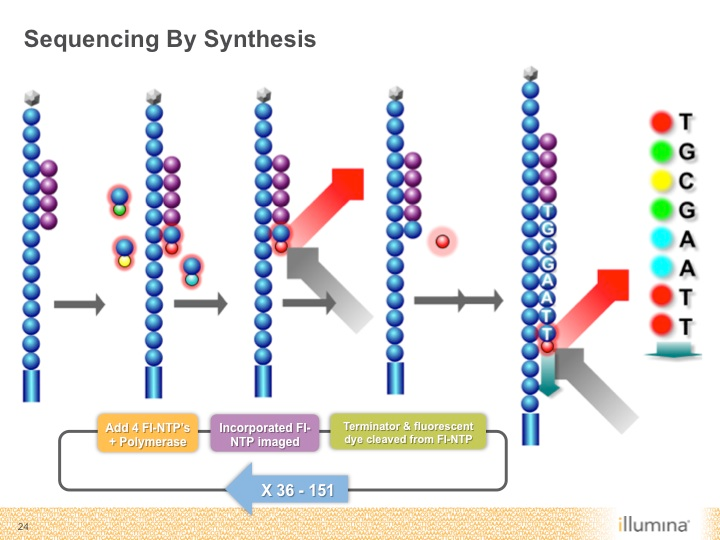
\includegraphics[width=0.5\textwidth]{illumina_fig.png}
  \end{center}
  \vspace{-20pt}
  \caption[Illumina]{Illumina \protect\cite{illuminafigure}}
  \vspace{-10pt}
  \label{fig:illumina}
\end{wrapfigure}

An advantage to this technology is its reliability. Because bases are incorporated into the sequence one at a time, the chance of the machine making an error when it reads and records the sequence is reduced. In addition, this reaction is particularly easy to mass-produce, which provides opportunities for greater efficiency. Another way to think about it is to consider Illumina as the "Costco" of DNA sequencers. If you sequence in bulk, you can reduce your costs.

\subsection{Ion Torrent}

Ion Torrent's process for sequencing DNA, called "semiconductor sequencing", is similar to Illumina, but with some key differences. Both begin by isolating a single DNA strand. Rather than introducing all four nucleotides at the same time, Ion Torrent only introduces one base at a time. When a nucleotide base-pairs to the DNA strand, it releases a hydrogen ion. In the Ion Torrent machine, there is a hypersensitive pH meter. It can detect the single addition of a hydrogen ion in a solution. If, when the nucleotide is introduced to the DNA strand, the machine does not detect a change in pH, that nucleotide is removed, and the next kind is brought in. The process is repeated until the machine detects a change in pH. When that happens, the computer records which base was incorporated and repeats the cycle until the sequencing is complete.

Because Ion Torrent doesn't need highly specialized reagents such as nucleotides with color-coded fluorophores, it is generally cheaper than most technologies. However, it does not benefit from an "economies of scale" as does Illumina. Additionally, Ion Torrent's machines are designed so that, as technology advances, the only upgrades ever needed are new semiconductor sequencing chips, rather than new machines entirely. This attribute makes Ion Torrent machines more appealing as long-run investments.

\subsection{PacBio}
This technology is referred to as "single-molecule, real-time DNA sequencing", or "SMRT sequencing." Its concept is also similar to that of Illumina and Ion Torrent, with its own important distinctions. SMRT sequencing begins by anchoring a single \textit{DNA polymerase} molecule to the bottom of a tiny well. Next, a single DNA strand is introduced to the DNA polymerase. In addition, all four kinds of nucleotides are added to the solution. These nucleotides have specifically colored fluorophores attached, as in Illumina. When DNA polymerase grabs the nucleotide that matches the DNA's sequence, it cleaves the fluorophore from the nucleotide, activating it in the process and emitting light (See Figure 2). A specialized camera recognizes the color of the light and records the respective base.

\begin{wrapfigure}{r}{0.6\textwidth}
\vspace{-20pt}
  \begin{center}
    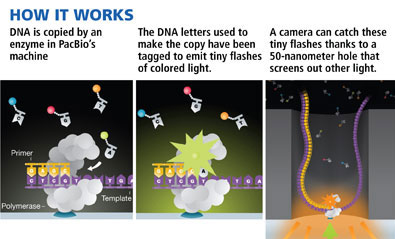
\includegraphics[width=0.48\textwidth]{pacbio_fig.png}
  \end{center}
  \vspace{-20pt}
  \caption[PacBio]{PacBio \protect\cite{pacbiofigure}}
  \vspace{-10pt}
  \label{fig:pacbio}
\end{wrapfigure}

The major advantage to this technology is DNA polymerase works extremely fast (around 1,000 base pairs per second) \cite{kelman}. This attribute allows PacBio to sequence DNA very quickly. However, it is not easily mass-produced because there can only be one DNA strand sequenced per well.

\subsection{Oxford Nanopore}

\begin{wrapfigure}{r}{0.6\textwidth}
\vspace{-30pt}
  \begin{center}
    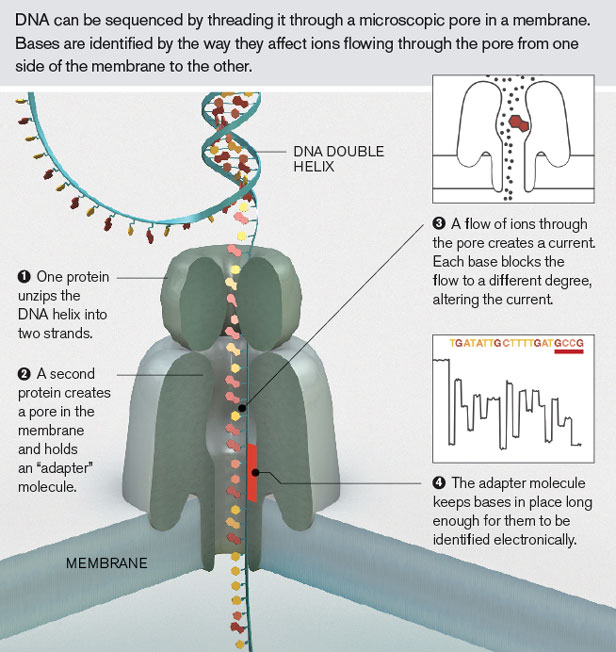
\includegraphics[scale=.5]{oxford_fig.png}
  \end{center}
  \vspace{-20pt}
  \caption[Oxford Nanopore]{Oxford Nanopore \protect\cite{oxfordfigure}}
  \vspace{-10pt}
  \label{fig:oxford}
\end{wrapfigure}

Oxford Nanopore utilizes "strand sequencing." The key to the workings of strand sequencing is a synthetically produced protein designed specifically for this task. This protein has a tube in the middle that is nanometers in diameter, making it small enough so only one strand of DNA can pass through at a time. This protein is also designed to fit into a tiny pore on a synthetic membrane. An electric current is then run through the membrane. Whenever anything passes through the small tube in the protein, it disrupts the current. Each molecule that passes through the protein creates its own distinct disruption. 

When a DNA strand, for example, is run through the protein, the disruptions made can be categorized into each of the four bases. In other words, the disruptions can be translated into the DNA's sequence (See Figure \ref{fig:oxford}) \cite{nanoporesite}. Ideally, because strand sequencing does not require any DNA synthesis and very few reagents, as do the other three technologies, it should be faster, more accurate, and cheaper \cite{Xuan}. Therefore, Oxford Nanopore is expected to be the most efficient of the sequencing technologies. To determine if this is true, we selected three parameters (cost per megabase, time per run, and output per run) to measure and compare each technology. 

\section{Methodology}

In order to accurately compare sequencers, we elected to compare each technology based on cost per megabase, time per run, and output per run. These metrics are a good measure of the efficacy of the machine and provide a solid foundation to allow us to make comparisons. We will now explain what each measurement is, why it was chosen, and how we obtained our data. In addition, we provide a "caveats" section describing some limitations of this comparison.

\subsection{Cost per Megabase}

Considering the fact that the Human Genome Project cost around \$2.7 billion dollars, the cost of sequencing is a major limiting factor when considering projects \cite{Salto-Tellez}. Utilizing technologies that sequence at lower costs enable researchers to take on bigger projects and obtain more data \cite{Shendure}. Therefore, the cost it takes to obtain one megabase (1 million bases) of data is heavily considered by researchers when choosing what kind of sequencing technology to use. In fact, it is used by the National Human Genome Research Institute in their widely known and important benchmark graphs illustrating the decreasing costs associated with DNA sequencing. This measurement captures all of the direct "production" costs of producing the raw sequencing data. These production costs include \cite{nhgriseqcosts}:

\begin{enumerate}
  \item Labor, administration, management, utilities, reagents, and consumables
  \item Sequencing instruments and other large equipment (amortized over three years)
  \item Informatics activities directly related to sequence production (e.g., laboratory information management systems and initial data processing)
  \item Shotgun library construction (required for preparing DNA to be sequenced)
  \item Submission of data to a public database
  \item Indirect Costs as they relate to the above items
\end{enumerate}

These are all important costs associated with producing DNA sequence data and should be captured in a cost per megabase measurement. We collected cost per megabase data for the established sequencers from van Dijk, Loman, and Mikheyev \cite{van_Dijk,Loman,Mikheyev} and data for the Oxford Nanopore from Quick \cite{Quick}.

The price of purchasing the actual sequencing machine is a critically important factor for those institutions looking to be able to sequence in-house. However, for others looking to outsource their DNA sequencing needs, this cost is not as important as the cost per megabase. For the scope of this report, we will refrain from incorporating the cost of the actual machines into our comparison.

\subsection{Time per Run}
	
Time per run is an indicator of how quickly a machine can turn DNA template into sequence data. Researchers hold this quality of high importance because, as of now, genomic sequencing takes a considerable amount of time to complete (the Human Genome Project, for example, took about 13 years) \cite{nhgrifaq}. Therefore, the shorter the run-time for sequencing, the quicker each project can be completed. This is a crucial consideration not only for researchers, but also for investors who are anxious for good returns in a timely manner. This information was found by combining data from Quick and van Dijk \cite{Quick, van_Dijk}.
     
\subsection{Output per Run}

Output per run is the number of base pairs sequenced in a single run on a machine. It is important to consider output per run alongside time per run because a machine with a short run-time is inefficient if it also produces a low output. In addition, a higher output per run increases efficiency in terms of cost. Each run of a machine costs a considerable amount of money, so the more output generated by each run, the more cost-efficient the machine. We used data from van Dijk, Loman, and Mikheyev for our analysis \cite{van_Dijk,Loman,Mikheyev}. 

\subsection{Caveats}

\subsubsection{Validity of Machine Comparison}

Each technology we have discussed comes in many forms. For example, Illumina sells four different kinds of machines that use the same technology, but are built for different purposes \cite{illuminasite}. We found that all but one of our chosen technologies offers a "desktop" machine, made to be efficient both in terms of money and time. However, these machines were not intended for use on large, data-intensive projects. Because the purpose of our report is to compare these technologies in terms of efficiency, and in an effort to be as unbiased as possible, we chose to use data collected from the desktop version of each technology. For Illumina, we used the MiSeq sequencer. For Ion Torrent, we used PGM, and for Oxford Nanopore, we used MinION.

One problem with this decision is that PacBio does not offer a desktop sequencer. Their only machine, the PacBio RS II, is noted for its high accuracy and long reads, but not necessarily efficiency \cite{pacbiosite}. While it would've been ideal to use data from a PacBio desktop unit, that was not possible, so we collected data for the RS II.

These circumstances reduce the validity of our comparison because the RS II was not built for the same purposes as the other three desktop sequencers. Despite this, we feel that given the situation, we have produced the best comparison possible to determine the most cost and time efficient technology.

\subsubsection{Sources of MinIon data}

Since the Oxford Nanopore technology is so new, there is significantly less data on its capabilities compared to the more established sequencers. The public's main source of unbiased data comes from a handful of published studies done by "early access" customers. The early access program allowed a small number of selected labs, institutions, and individuals to purchase an Oxford Nanopore sequencer in early spring 2014. Some of these groups went on to do small sequencing projects using the MinION, usually sequencing small bacterial genomes, and publishing the results. Besides giving a brief but useful explanation of the MinION sequencer itself, these studies provide unbiased information on the data this machine produces and represent our main source of information regarding the price, speed, and output of this technology. The disadvantage of this source is that it uses a small sample size. Due to the MinION's novelty, not many programs have tested it to provide results. In the future, there are sure to be more reliable sources with MinION data, but for our time frame, this was the best option. 

\subsubsection{Variability of MinION results}

The results of a sequencing run can vary by a lot of factors. Because MinION is such a new technology, many of its protocols and reagents are in flux. This is especially true of the critical flow cells that form the basic consumable reagent of the MinION. Early access users were given a generation of flow cells called R6. Within a short time, improvements were applied, and versions R7 (released in July 2014) and R7.3 (released in September 2014) were made available. 

The advanced chemistry of these flow cells, while outside the scope of this report, plays a huge role in the quality of the results. This is demonstrated by certain studies, which used the older R6 technology, and concluded that the results of Oxford Nanopore sequencing are so error prone that the technology is practically useless, yet others using the R7 technology were able to produce vastly improved results \cite{Mikheyev}. We provide a table (Table \ref{table:summary_nanopore}) showing the average results of a study which implemented the most recent iterations of the flow cell technology: The R7 and R7.3 \cite{Quick}.

\begin{table}[htb]
\begin{center}
\begin{tabular}{lll}
\hline
 & R7 & R7.3 \\
\hline
Run Time & 72 hr & 48 hr \\
template reads & 43,656 (272Mb) & 39,819 (163 Mb) \\
complement reads & 23,338 (125 Mb) & 18,889 (84 Mb) \\
2D reads & 20,087 (131 Mb) & 11,823 (64.53 Mb) \\
Read Length (2D) & 6,543 & 5,458 \\
\hline
\end{tabular}
\caption{MinIon results of older R7 flow cell vs. newer R7.3.}
\label{table:summary_nanopore}
\end{center}
\end{table}

\section{Data Summary}

\subsection{Cost per Megabase}

\begin{wrapfigure}{r}{0.6\textwidth}
\vspace{-20pt}
  \begin{center}
    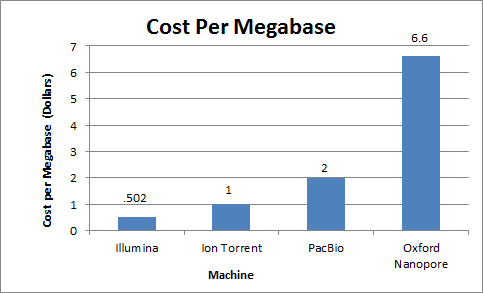
\includegraphics[width=0.6\textwidth]{cost_per_megabase.png}
  \end{center}
  \vspace{-20pt}
  \caption[Cost per Megabase]{Cost per Megabase \protect\cite{Quick}}
  \vspace{-10pt}
  \label{fig:cost_per_megabase}
\end{wrapfigure}

Figure \ref{fig:cost_per_megabase} displays our results for cost per megabase of sequenced data. The Oxford Nanopore cost was calculated using the reported flow cell price of \$1,000 and dividing it by the average output per run, which is 150 Mb \cite{Quick}. As evidenced from Figure \ref{fig:cost_per_megabase}, Oxford Nanopore produces the most expensive reads by a factor of at least 3 when compared to the other machines. Illumina had the cheapest cost per megabase at around 50 cents per million bases. This means that a human genome (3,000 Mb) could be sequenced for around \$1,500 using Illumina, whereas Oxford Nanopore would cost \$19,800.

\subsection{Time per Run}

\begin{wrapfigure}{r}{0.6\textwidth}
  \vspace{-20pt}
  \begin{center}
    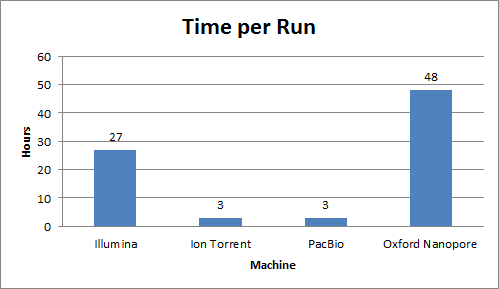
\includegraphics[width=0.6\textwidth]{time_per_run.png}
  \end{center}
  \vspace{-20pt}
  \caption[Time per Run]{Time per Run \protect\cite{Quick,van_Dijk}}
  \vspace{-10pt}
  \label{fig:time_per_run}
\end{wrapfigure}

The data we compiled for time per run are shown in Figure \ref{fig:time_per_run}, where time is measured in hours. We see that Oxford Nanopore has the longest time per run by 78\% (when compared to Illumina). Oxford Nanopore also takes 15 times longer than Ion Torrent and PacBio. While this measurement does serve as an indicator for efficiency in terms of time, it must also be considered in conjunction with output per run to determine true efficiency. We will discuss output per run next. 

\subsection{Output per Run}

\begin{wrapfigure}{r}{0.6\textwidth}
\vspace{-20pt}
  \begin{center}
    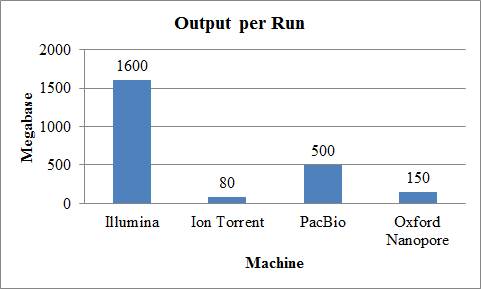
\includegraphics[width=0.6\textwidth]{output_per_run.png}
  \end{center}
  \vspace{-20pt}
  \caption[Output per Run]{Output per Run \protect\cite{Quick,van_Dijk,Loman,Mikheyev}}
  \vspace{-10pt}
  \label{fig:output_per_run}
\end{wrapfigure}

Output per run is measured in megabases (Mb) of data. The results of our research can be seen in Figure \ref{fig:output_per_run}. We found that Illumina has the highest output per run, being more than three times larger than PacBio, more than ten times larger than Oxford Nanopore, and about twenty times larger than Ion Torrent. In our discussion, we will consider time per run and output per run together in order to develop a more holistic analysis of efficiency.

\section{Discussion}

To interpret our results, we combined our data found for time per run and output per run to create a new measurement, throughput, or output per hour, measured in megabases. We did this by multiplying the inverse of our time per run statistics by output per run as shown in Figure \ref{fig:throughput_eq} below:

\begin{figure}[hr] %{0.5\textwidth}
  \begin{center}
    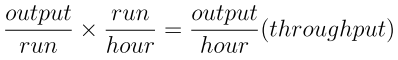
\includegraphics[width=0.5\textwidth]{throughput_eq.png}
  \end{center}
  %\vspace{-20pt}
  \caption{Throughput Equation}
  \vspace{-10pt}
  \label{fig:throughput_eq}
\end{figure}

The results from these calculations are shown in Figure \ref{fig:throughput_per_hour}. This interpretation suggests that PacBio is by far the most efficient in terms of time and productivity, delivering 166.67 megabases of sequencing data per hour. Oxford Nanopore definitely underperforms in this category, producing a mere 3.13 megabases of sequencing data per hour. 

\begin{figure}[hr] %{0.5\textwidth}
  \begin{center}
    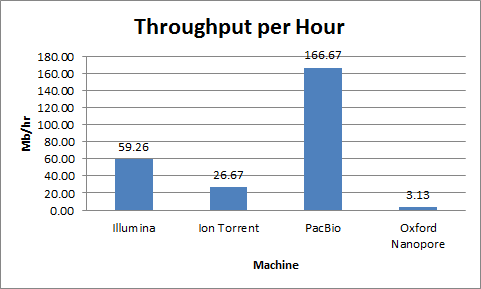
\includegraphics[width=0.6\textwidth]{throughput_per_hour.png}
  \end{center}
  %\vspace{-20pt}
  \caption{Throughput (Output per hour)}
  \vspace{-10pt}
  \label{fig:throughput_per_hour}
\end{figure}

Having determined the most productive and expeditive machine, we will now discuss the machine that is the most efficient in terms of cost. Referring back to Figure \ref{fig:cost_per_megabase}, we see that Illumina is the most cost efficient, costing only .502 dollars to sequence one million bases, with Oxford Nanopore, once again, as the least efficient, costing \$6.60 to sequence one million bases. As mentioned before, this seemingly small price difference is very significant when sequencing billions of bases.

From this analysis, we have determined that Illumina's MiSeq is more efficient in terms of cost, and PacBio's RS II is more efficient in terms of time. However, the aim of this report is to determine the most overall efficient machine. To accomplish this, we will compare the degrees to which each is the most efficient. From our data, we calculated ratios of each measurement and determined that Illumina is 3.98 times more cost-efficient than PacBio, whereas PacBio's throughput is only 2.81 times larger than Illumina. Next, we will take these interpretations and formulate our conclusion. 

\section{Conclusion}

In this report, we aim to determine if Oxford Nanopore deserves the hype it's receiving by the media and if it's desktop MinION unit is more efficient in terms of money, time, and output than the leading desktop DNA sequencing machines. If it is not, then we aim to determine which machine is the most efficient. To determine this, we gathered research on four technologies (Illumina, Ion Torrent, PacBio, and Oxford Nanopore). We compiled statistics of cost per megabase, time per run, and output per run. From these data, we combined time per run and output per run to generate a new measurement, throughput, or output per hour. Our analysis of throughput indicated to us which machine was the most efficient in terms of time and productivity, and cost per megabase indicated to us which machine was the most efficient in terms of money.

From our analysis, we conclude that Oxford Nanopore is far from being more efficient than the other leading technologies. In fact, it is, by a large margin, the least efficient of those that we compared. Because of this result, we have also determined which of the current technologies is the leader in efficiency.

We conclude that Illumina provides the most overall efficient desktop machine (MiSeq).
Even though PacBio has a higher throughput, its sequencing cost is four times more than Illumina. In practice, this means that while PacBio can sequence a human genome in 18 hours (50 hours for Illumina), it would cost \$6,000 to do so compared to about \$1,500 for Illumina.

As the field of genomics grows, many researchers and institutions around the world are considering investing in a DNA sequencing machine. This research can be of great value to those who are considering purchasing Oxford Nanopore's MinION unit because of all the public hype the machine is receiving. However, we find that they will save a lot more time and money if they instead invest in purchasing Illumina's MiSeq unit.

Although our results indicate that the Oxford Nanopore technology is not up to par with the standard sequencing technologies yet and may have prematurely received praises from the media, we still believe it has unrealized potential. The fundamental design utilizing a synthetic protein that allows for a straight read of DNA rather than reading the sequence by synthesis is miles ahead of the technology currently being used. We believe that the advantages from this technology will become more apparent as the process is developed and refined. In fact, all of the established technologies that we compared Oxford Nanopore to went through a development period of their own before they became the reliable machines they are today. Still, these development periods typically take years or even decades. While we would not recommend purchasing the MinION unit now or even in a few years, we also advise our readers to keep a close eye on its development, for it may one day result in the most powerful and efficient DNA sequencer the world has seen yet.

Thank you for reading our report. If there are any questions, comments, or clarifications, we can be contacted by email at any of these addresses: mollyloschiavo@gmail.com, kevinlboehme@gmail.com, coric8@gmail.com.


% The bibtex filename
\addcontentsline{toc}{chapter}{References}
\bibliography{references}
\clearpage

%Appendix
\addcontentsline{toc}{chapter}{Appendix}
\begin{center}
\vspace*{\fill}
\Huge\textbf{Appendix}
\vspace*{\fill}
\end{center}
\clearpage

\setcounter{section}{0}
%Glossary
\addcontentsline{toc}{chapter}{Glossary}
\begin{center}
\Huge\textbf{Glossary}
\end{center}

\textbf{\textit{Base-pair}}: A chemical bond between two nucleotides. A and T bond exclusively, and C and G bond exclusively. DNA is naturally found in a state where all of it's nucleotides are base-paired to the nucleotides of another DNA strand. This term is often interchangeable with "nucleotide" and "base".

\textbf{\textit{DNA}}: Deoxyribonucleic acid. A molecule whose sequence of nucleotides (see below) contains the information a cell needs to produce all proteins necessary for survival. Each cell in the human body contains a complete set of these "instructions". 

\textbf{\textit{DNA polymerase}}: Enzyme (protein) that dramatically increases the speed of the nucleotide base-pairing process by matching each base in a DNA strand with it's complementary base and creating the bond that holds the two bases together. 

\textbf{\textit{Flow cells}}: A consumable reagent for the Oxford Nanopore MinION that contains all components necessary for one "sequencing run". Houses the chemistry and nanopores needed to sequence and produce the DNA data.

\textbf{\textit{Fluorophore}}: Molecule that fluoresces a particular color when activated. Can be activated by a laser (as in Illumina) or by DNA polymerase (as in PacBio). In sequencing, particular colors of fluorophores are attached to particular bases. For example, all C's may be attached to red fluorophores, all T's may be attached to green fluorophores, all G's may be attached to blue fluorophores, and all A's may be attached to yellow fluorophores. 

\textbf{\textit{Genome}}: The entire DNA sequence found in an organism's cell. Contains all the information for creating, growing, and sustaining that organism. The human genome is around 3 billion base pairs long. 

\textbf{\textit{Megabase}}: One million base-pairs. Used as a unit of measurement for how many bases were sequenced. 

\textbf{\textit{Next-generation DNA sequencing technologies}}: Series of DNA sequencing technologies that emerged in the 1990's and new millennium in response to the Human Genome Project. These technologies vastly outperform those that had been used before this time, which is why they were considered to be a whole new generation. 

\textbf{\textit{Nucleotide}}: A building block of DNA. Also known as a "base" or "base pair". There are four kinds: A, G, C, and T. The order of nucleotides determines the DNA's sequence.

\textbf{\textit{Throughput}}: Output per hour given in Megabases/hour produced by a DNA sequencer. Helpful metric to compare sequencing technologies, indicating productivity.

\clearpage

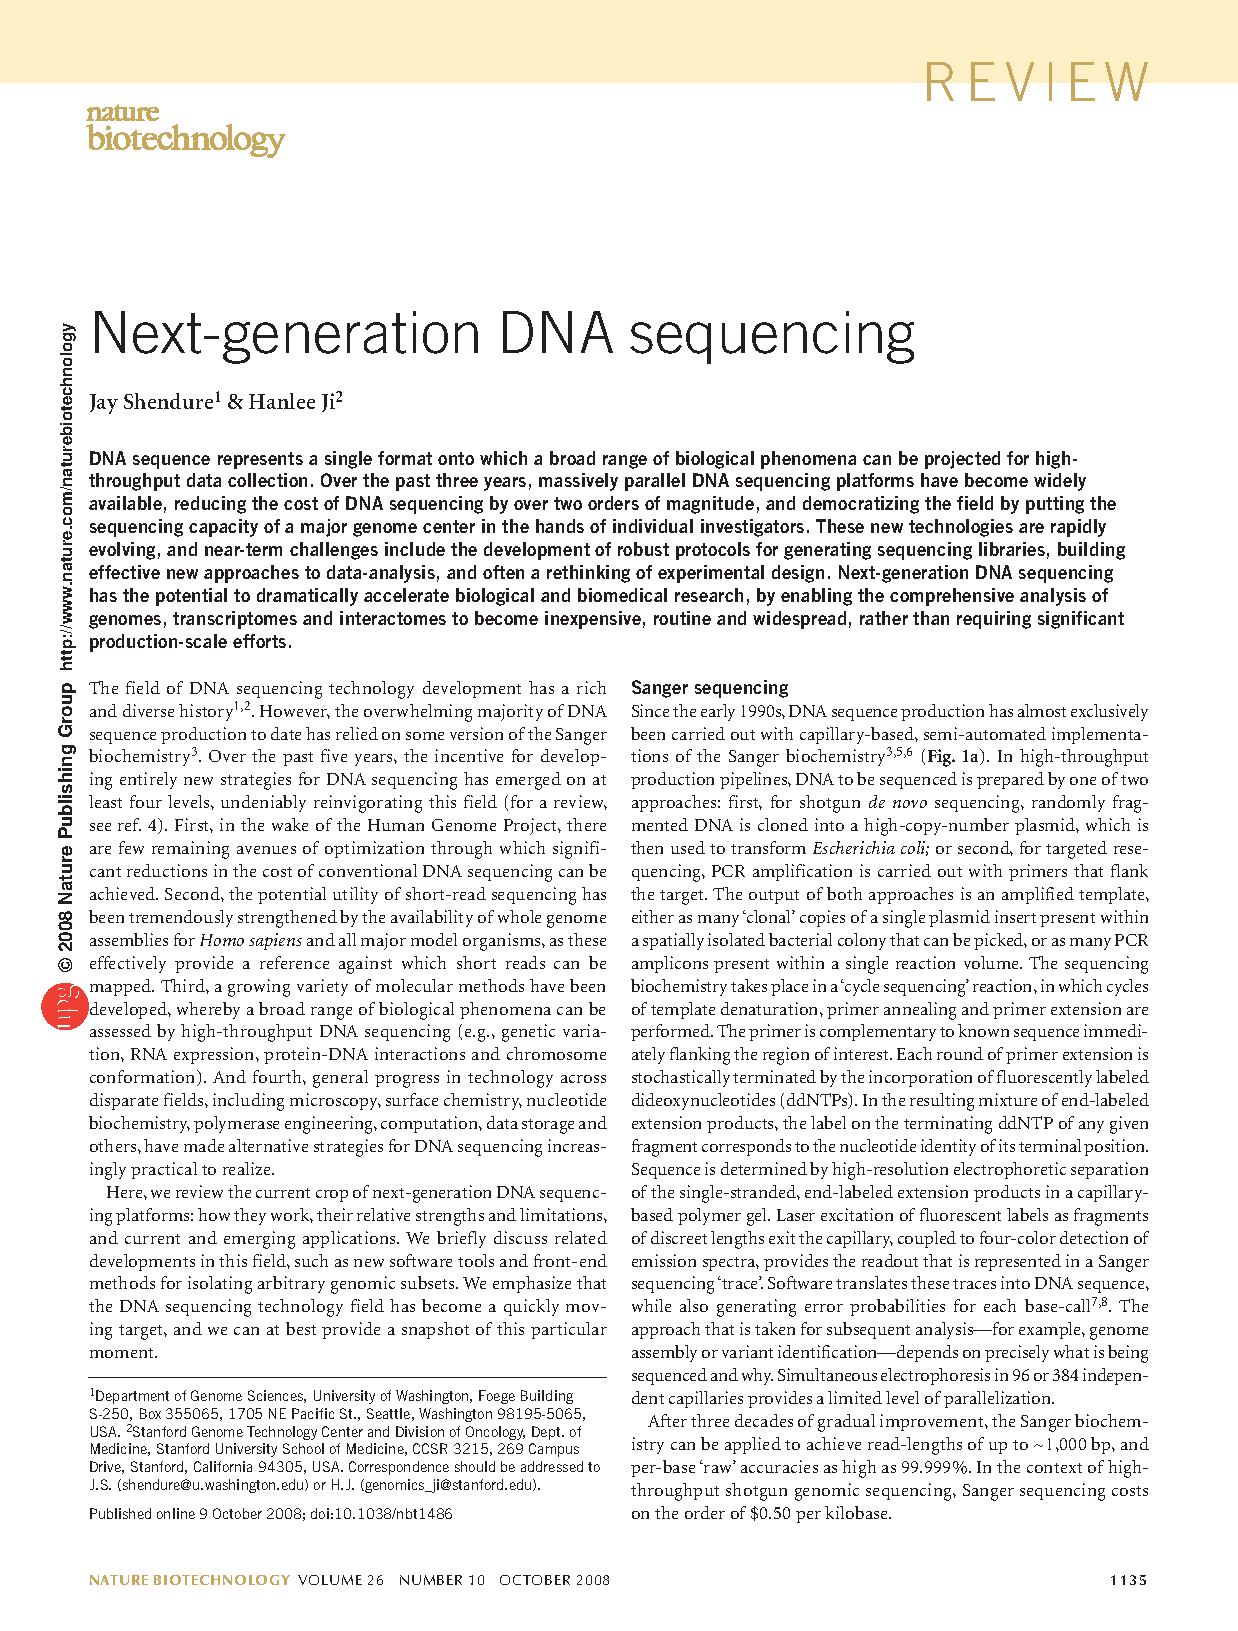
\includepdf[pages={-}]{ref_format.pdf}

\end{document}